
% This LaTeX was auto-generated from MATLAB code.
% To make changes, update the MATLAB code and republish this document.

\documentclass{article}
\usepackage{graphicx}
\usepackage{color}

\sloppy
\definecolor{lightgray}{gray}{0.5}
\setlength{\parindent}{0pt}

\begin{document}

    
    
\section*{Zachary Kaplan}

\begin{par}
Math 440 Computational Lab \#2 2/27/19
\end{par} \vspace{1em}
\begin{par}
An online version of this file can be found published to: https://www.overleaf.com/read/qmtzkncjftck
\end{par} \vspace{1em}
\begin{par}
\textbf{NOTE}: To render this file locally, please prepend the following package         dependencies to the latex generated by matlab publish:
\end{par} \vspace{1em}

\begin{verbatim}\usepackage[margin=1in]{geometry}
\usepackage{amsmath}
\usepackage{amssymb}
\usepackage{microtype}
\usepackage{csquotes}
\usepackage{bm}\end{verbatim}
    
\subsection*{Contents}

\begin{itemize}
\setlength{\itemsep}{-1ex}
   \item Numerical Scheme
   \item Van der Pol's DE
   \item C.2.1.1 Accuracy of our RK-3 Method
   \item Robertson's Problem
   \item C.2.1.2 Stability Investigation of our RK-3 Method
   \item C.2.1.2.1 RK-3 w/ fixed grid size.
   \item C.2.1.2.2 Stability w/ Adaptive Time-Stepping
   \item C.2.1.3 Parameter Study of an ODE System
   \item C.2.1.3.1 Particle Flow Past a Cylinder
   \item C.2.1.3.2 Motion of a Particle
   \item Functions Used Above
   \item RK-3 Solver
   \item RK-4 Solver
\end{itemize}


\subsection*{Numerical Scheme}

\begin{par}
In this lab, we will consider the following explicit RK-3 scheme on a system of the form $u_t = f(t, u)$:
\end{par} \vspace{1em}
\begin{par}
$$ \begin{aligned}
  u_k &=
    u_{k-1} + \frac{h}{6}\left(K^{(k)}_1 + K^{(k)}_2 + 4K^{(k)}_3\right),
    \quad t_k = t_{k-1} + h,
    \quad k \in 1, 2, \ldots, N \\
  K^{(k)}_1 &= f\left(t_{k-1}, u_{k-1}\right) \\
  K^{(k)}_2 &= f\left(t_{k-1} + h, u_{k-1} + hK^{(k)}_1\right) \\
  K^{(k)}_3 &=
    f\left(t_{k-1} + h/2, u_{k-1} + h/4\left[
      K^{(k)}_1 + K^{(k)}_2 \right]\right) \\
\end{aligned} $$
\end{par} \vspace{1em}


\subsection*{Van der Pol's DE}

\begin{par}
For the first section of this lab, we will consider the following non-linear differential equation:
\end{par} \vspace{1em}
\begin{par}
$$
  \frac{d^2 y}{dt^2} + (y^2-1)\frac{dy}{dt} + y = 0,
    \quad y(0) = 1, \frac{dy}{dt}(0) = 0,
    \quad t \in [0, 1]
$$
\end{par} \vspace{1em}
\begin{par}
Using the substitution $x = y_t$, we can rewrite the above as the following coupled system of ODEs:
\end{par} \vspace{1em}
\begin{par}
$$ \left\{ \begin{aligned}
  x_t &= (1-y^2) x - y \\
  y_t &= x
\end{aligned} \right. $$
\end{par} \vspace{1em}
\begin{par}
Therefore, if we define the vector $\bm{X} = \begin{pmatrix} x \\ y \end{pmatrix}$, we can describe Van der Pol's equation as $\bm{X}_t = f(t, \bm{X})$ where
\end{par} \vspace{1em}
\begin{par}
$$
  f\left(t, \bm{X}\right) =
    \begin{pmatrix} (1-y^2)x - y \\ x \end{pmatrix}.
$$
\end{par} \vspace{1em}


\subsection*{C.2.1.1 Accuracy of our RK-3 Method}

\begin{par}
In order to numerically estimate the order of our method on the Van der Pol model, we will consider partitions of sizes $N = 10, 20, 40, 80, 160, 320$ over the support $t \in [0, 1]$. If we write $y^{(N)}$ to be the numerical solution to Van der Pol's equation with partition size $N$, then we can calculate the error at $t = 1$ for that partition size as $e_N = y^{(N)}_N - y(1)$. Since the true value of $y(1)$ is unknown, consider $y^{(320)}_{320}$ to be a good enough approx to $y(1)$ and use that to find the errors $e_N$ for $N = 10, 20, 40, 80, 160$.
\end{par} \vspace{1em}
\begin{verbatim}
% Partition sizes to consider.
N = pow2(10, 0:5);
% Support interval to consider.
T_int = [0, 1];
% Initial value of X = [ y' ; y ] at t = 0.
X_0 = [0 ; 1];
% RHS of the coupled ODE for Van der Pol's equation.
% NOTE: The first argument, t, is ignored because f is autonomous.
f = @(~, X) [ (1 - X(2)^2)*X(1) - X(2) ; X(1) ];

% Consider solution for N = 320 to be `exact'.
X_true = rk3_solve(f, X_0, T_int, N(end));
X_true = X_true(:, end);  % We only need the final value at t = 1.

% Allocate space for the approximate error of the other solutions.
err = zeros(length(X_true), length(N) - 1);
% Allocate space for the grid spacing of each method.
h = zeros(1, length(N) - 1);

% Solve for each N except the last one.
for i = 1:(length(N)-1)
    [X, ~, h(i)] = rk3_solve(f, X_0, T_int, N(i));
    err(:, i) = X(:, end) - X_true;
end

% Now plot the magnitude of the error in y by h.
% NOTE: y is the second component of X.
figure;
loglog(h, abs(err(2, :)), '-x');
set(gca, 'XDir', 'reverse')  % Display h's decreasing left-to-right.
xlabel('Grid Spacing h = 1/(N-1)')
ylabel('Error |e_N|')
title({'C.2.1.1', 'Approximate Error vs. Grid Spacing'})

% Approximate the order as the slope of the above graph.
% Using the first and last point to approximate the slope.
order = abs(log(err(2, end)) - log(err(2, 1))) / ...
            abs(log(h(end)) - log(h(1)));
% Print the order on the graph.
annotation('textbox', [.55 .55 .1 .1], 'LineStyle', 'none', ...
           'Interpreter', 'latex', ...
           'String', sprintf('Order $\\approx %.2f$', order))
\end{verbatim}

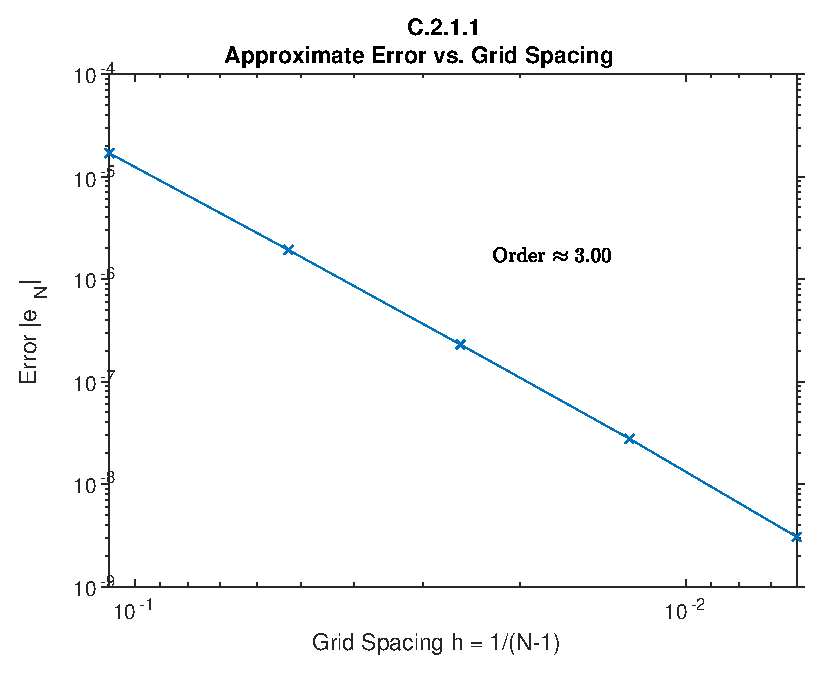
\includegraphics [width=4in]{lab2_01.eps}


\subsection*{Robertson's Problem}

\begin{par}
For the next section, we will consider the following coupled nonlinear ODE's which form a stiff problem:
\end{par} \vspace{1em}
\begin{par}
$$ \left\{ \begin{aligned}
  \frac{dx_1}{dt} &= -k_1 x_1 + k_2 x_2 x_3, & x_1(0) = 1 \\
  \frac{dx_2}{dt} &= k_1 x_1 - k_2 x_2 x_3 - k_3 x_2^2, & x_2(0) = 0 \\
  \frac{dx_3}{dt} &= k_3 x_2^2, & x_3(0) = 0
\end{aligned} \right. $$
\end{par} \vspace{1em}
\begin{par}
where $k_1 = 0.04, k_2 = 10^4, k_3 = 3 \cdot 10^7$. The above is trivially vectorized by considering $\bm{X} = \begin{pmatrix} x_1 & x_2 & x_3 \end{pmatrix}$.
\end{par} \vspace{1em}


\subsection*{C.2.1.2 Stability Investigation of our RK-3 Method}

\begin{par}
Below we will examine the stability of our RK-3 method as well as the stability of some of matlab's built-in solvers.
\end{par} \vspace{1em}


\subsection*{C.2.1.2.1 RK-3 w/ fixed grid size.}

\begin{par}
Below we consider Robertson's problem for $t \in [0, 1]$, and grid sizes of $N = 125, 250, 500, 1000, 2000$. We will then (qualitiatively) classify the behavior for different $N$ values to determine at which minimal $N$ value the solution becomes stable.
\end{par} \vspace{1em}
\begin{verbatim}
% Support interval to consider.
T_int = [0, 1];
% N values to consider.
N = pow2(125, 0:4);
% Initial value of X at t = 0.
X_0 = [ 1 ; 0 ; 0 ];

% Constants k_{1, 2, 3}.
k = [ 0.04, 10^4, 3*10^7 ];
% RHS of ODE.
f = @(~, X) [ -k(1)*X(1) + k(2)*X(2)*X(3) ; ...
              k(1)*X(1) - k(2)*X(2)*X(3) - k(3)*X(2)^2 ; ...
              k(3)*X(2)^2 ];

% Allocate storage for each solution. We use a cell array to represent
% multiple solutions and their supports.
XN = cell(size(N));
TN = cell(size(N));
% Compute each solution and store it in the cell array.
for i = 1:length(N)
    [XN{i}, TN{i}] = rk3_solve(f, X_0, T_int, N(i));
    % Print out the value of the solution at t = 1 for qualitative
    % comparison.
    fprintf('N = %4d, X(1) = ( %f, %f, %f )^T\n', N(i), XN{i}(:, end));
end
\end{verbatim}
\begin{par}
By inspection of the output of the above, we notice that the solution exceeds the bounds of IEEE double precision floats until $N \ge 1000$. Since this problem is physical, we expect that the solution should NOT grow greater than $\approx2^{300}$ and therefore notice that the solution behaves stable (bounded) for $N \ge 1000$.
\end{par} \vspace{1em}
\begin{par}
We now plot the trajectory of each $x_i$ over time for $N = 1000$.
\end{par} \vspace{1em}
\begin{verbatim}
% Get the support and solution where N = 1000.
min_N = 1000;
X = XN{N == min_N};
T = TN{N == min_N};

% Plot each x_i in it's own subplot.
figure
for i = 1:3
    subplot(3, 1, i);
    loglog(T, X(i, :));
    ylabel(sprintf('Values of x_%d', i));
    title(sprintf('Approximate Solution of x_%d', i));
end

% Only put an xlabel on the last plot to be less redundant.
xlabel('t');
% Title for whole grid.
sgtitle({'C.2.1.2.1', sprintf('Approximate Solution with N = %d', min_N)});
\end{verbatim}


\subsection*{C.2.1.2.2 Stability w/ Adaptive Time-Stepping}

\begin{par}
First we will look at results for the non-stiff solver ode23 on $[0, 1]$, using $RelTol = 10^{-3}, 10^{-4}, 10^{-5}, 10^{-6}$. We'll then plot h(t) for the final tolerance.
\end{par} \vspace{1em}
\begin{verbatim}
fprintf('\nUsing ode23:\n')

% NOTE: Values of T_int, X_0, and f are still valid from prev. subsection.
rel_tol = power(10, -(3:6));
X_by_tol = cell(size(rel_tol));
T_by_tol = cell(size(rel_tol));

% Solve for each tolerance.
for i = 1:length(rel_tol)
    [T_by_tol{i}, X_by_tol{i}] = ...
        ode23(f, T_int, X_0, odeset('RelTol', rel_tol(i)));
    % Print out # of steps taken for the given tolerance.
    fprintf('RelTol = %.0e, # of steps = %d\n', ...
            rel_tol(i), length(T_by_tol{i}));
end

% Pick the last T to plot.
T = T_by_tol{end};

% Plot.
figure
% Plot the difference in t values (h) vs. the T values.
plot(T(2:end), diff(T))
ylabel('h (step size)')
xlabel('t')
title({'C.2.1.2.2', 'Step Size (h) vs. Time (t) - ode23'})
\end{verbatim}
\begin{par}
Next we will run the stiff ODE solver ode23s for $t \in [0, 1000]$, and do the same as the above.
\end{par} \vspace{1em}
\begin{verbatim}
fprintf('\nUsing ode23s:\n')

% Preallocate for X and T.
X_by_tol = cell(size(rel_tol));
T_by_tol = cell(size(rel_tol));

% Solve for each tolerance.
for i = 1:length(rel_tol)
    [T_by_tol{i}, X_by_tol{i}] = ...
        ode23s(f, T_int, X_0, odeset('RelTol', rel_tol(i)));
    % Print out # of steps taken for the given tolerance.
    fprintf('RelTol = %.0e, # of steps = %d\n', ...
            rel_tol(i), length(T_by_tol{i}));
end

% Pick the last T to plot.
T = T_by_tol{end};

% Plot.
figure
% Plot the difference in t values (h) vs. the T values.
plot(T(2:end), diff(T))
ylabel('h (step size)')
xlabel('t')
title({'C.2.1.2.2', 'Step Size (h) vs. Time (t) - ode23s'})
\end{verbatim}

        \color{lightgray} \begin{verbatim}N =  125, X(1) = ( NaN, NaN, NaN )^T
N =  250, X(1) = ( NaN, NaN, NaN )^T
N =  500, X(1) = ( NaN, NaN, NaN )^T
N = 1000, X(1) = ( 0.966460, 0.000031, 0.033510 )^T
N = 2000, X(1) = ( 0.966460, 0.000031, 0.033510 )^T

Using ode23:
RelTol = 1e-03, # of steps = 867
RelTol = 1e-04, # of steps = 868
RelTol = 1e-05, # of steps = 869
RelTol = 1e-06, # of steps = 869

Using ode23s:
RelTol = 1e-03, # of steps = 17
RelTol = 1e-04, # of steps = 17
RelTol = 1e-05, # of steps = 17
RelTol = 1e-06, # of steps = 17
\end{verbatim} \color{black}
    
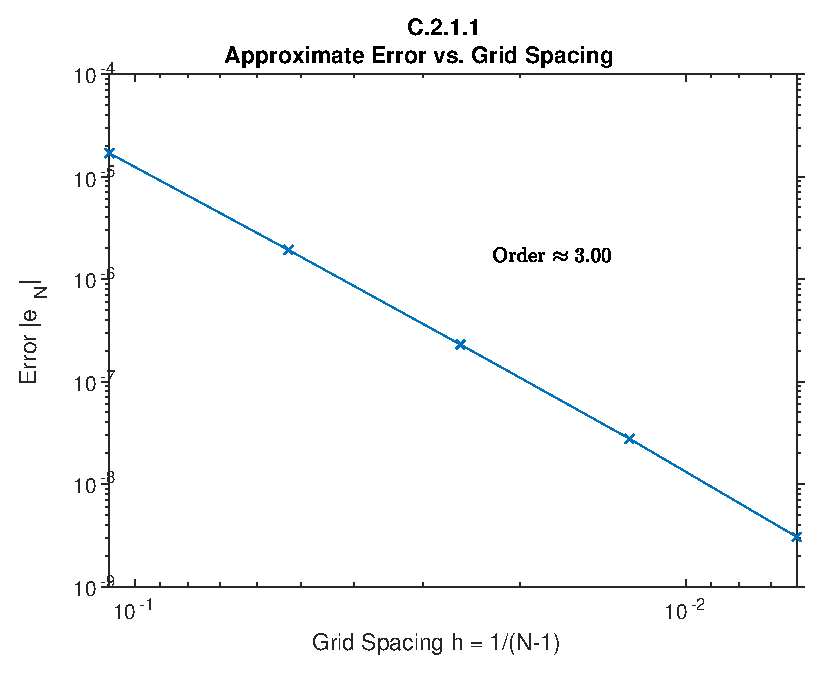
\includegraphics [width=4in]{lab2_02.eps}

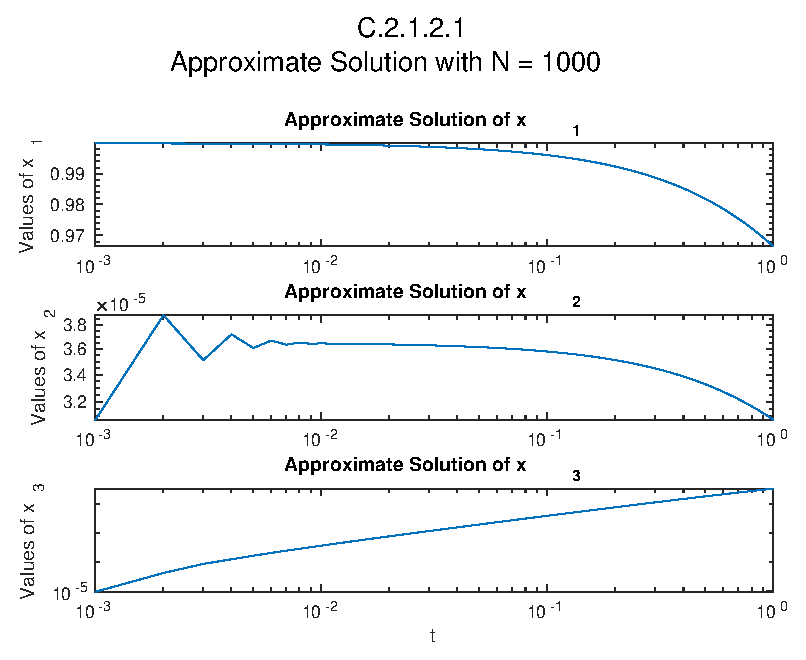
\includegraphics [width=4in]{lab2_03.eps}

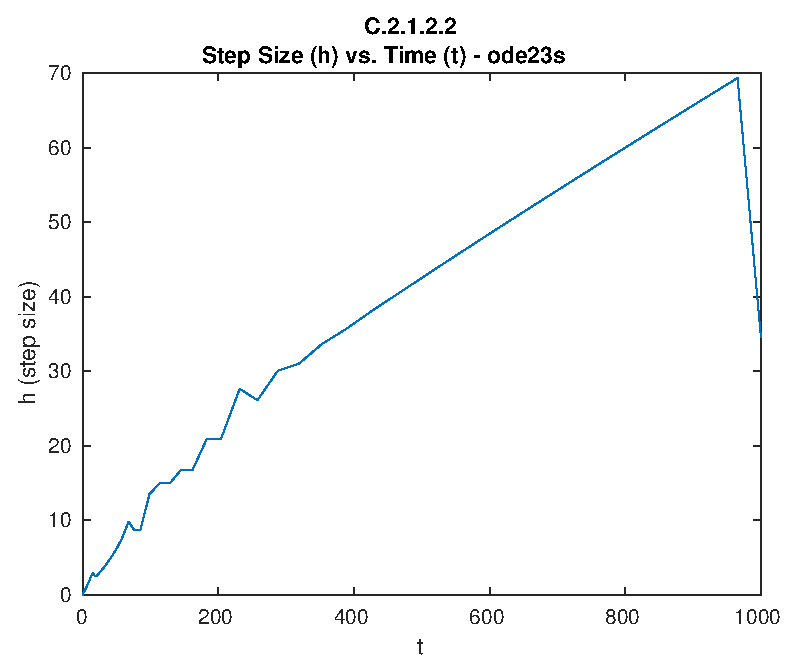
\includegraphics [width=4in]{lab2_04.eps}

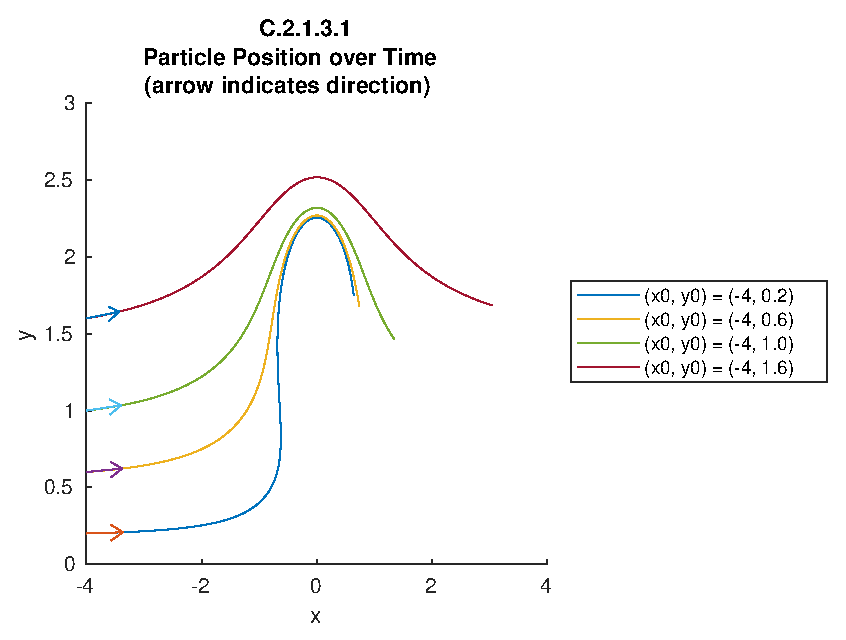
\includegraphics [width=4in]{lab2_05.eps}


\subsection*{C.2.1.3 Parameter Study of an ODE System}

\begin{par}
For the following ODEs, we will use the classical explicit RK-4 ODE solver to find numerical solutions, and then visualize qualitative changes in the numerical solutions as certain parameters are varied.
\end{par} \vspace{1em}


\subsection*{C.2.1.3.1 Particle Flow Past a Cylinder}

\begin{par}
The position of a particle is determined uniquely by it's initial point $(x(0), y(0))$ and
\end{par} \vspace{1em}
\begin{par}
$$ \left\{ \begin{aligned}
  x_t &= 1 - \frac{R^2(x^2-y^2)}{(x^2+y^2)^2} \\
  y_t &= - \frac{2xyR^2}{(x^2+y^2)^2)}
\end{aligned} \right. $$
\end{par} \vspace{1em}
\begin{par}
where we fix the radius of the cylinder to $R = 2$.
\end{par} \vspace{1em}
\begin{par}
Consider 4 particles starting at $x = -4$ and $y = 0.2, 0.6, 1.0, 1.6$. We then plot the flow of each particle in $\mathbb{R}^2$ for $t \in [0, 10]$.
\end{par} \vspace{1em}
\begin{verbatim}
% Set R = 2.
R = 2;

% We will consider X = [ x ; y ], and let each column i of the below denote
% the initial starting point of particle i.
X0s = [  -4  -4  -4  -4 ; ...
        0.2 0.6 1.0 1.6 ];
T_int = [0, 10];
f = @(~, X) [ 1 - R^2*(X(2)^2 - X(1)^2) / sum(X.^2)^2 ; ...
              - 2*prod(X)*R / sum(X.^2)^2 ];

% Preallocate solution space for each particle.
Xs = cell(1, size(X0s, 2));

% Solve for each particle.
for i = 1:size(X0s, 2)
    [Xs{i}, T] = rk4_solve(f, X0s(:, i), T_int, pow2(10));
end

figure
hold on;
% Preallocate for plot objects.
plots = zeros(1, length(Xs));
% Plot each particle's trajectory.
for i = 1:length(Xs)
    % First just plot the the actual path.
    plots(i) = plot(Xs{i}(1, :), Xs{i}(2, :), 'DisplayName', ...
                    sprintf('(x0, y0) = (%.0f, %.1f)', X0s(:, i)));
    % Now plot a single vector on the path indiciating direction.
    xy = Xs{i}(:, 1);
    uv = Xs{i}(:, floor(length(T)/20)) - xy;
    quiver(xy(1), xy(2), uv(1), uv(2), 0, 'MaxHeadSize', 100);
end
legend(plots, 'Location', 'EastOutside');
ylabel('y')
xlabel('x')
axis square;
title({'C.2.1.3.1', 'Particle Position over Time', ...
       '(arrow indicates direction)'})
\end{verbatim}


\subsection*{C.2.1.3.2 Motion of a Particle}

\begin{par}
Consider a particle thrown from (0, 1.5) at angle $\alpha$ and velocity $\nu_0 = 20$. The trajectory then depends on $\alpha$, the air resistance coefficient $k$, and the ODE system
\end{par} \vspace{1em}
\begin{par}
$$ \left\{ \begin{aligned}
  \frac{d^2x}{dt^2} &= -k\frac{dx}{dt}\sqrt{
     \left(\frac{dx}{dt}\right)^2 + \left(\frac{dy}{dt}\right)^2},
     && x(0) = 0, && \frac{dx}{dt}(0) = \nu_0 \cos(\alpha) \\
  \frac{d^2y}{dt^2} &= -g - k\left|\frac{dy}{dt}\right|\sqrt{
     \left(\frac{dx}{dt}\right)^2 + \left(\frac{dy}{dt}\right)^2},
     && y(0) = 1.5, && \frac{dy}{dt}(0) = \nu_0 \sin(\alpha)
\end{aligned} \right. $$
\end{par} \vspace{1em}
\begin{par}
where $g \approx 9.81$.
\end{par} \vspace{1em}
\begin{par}
We seek to solve this system with $\alpha = 30^\circ, 45^\circ, 60^\circ$ and $k = 0.020, 0.065$ and visualize the differences.
\end{par} \vspace{1em}
\begin{verbatim}
% Parameter values to consider.
nu_0 = 20;
g = 9.81;
alpha_deg = [30, 45, 60];
alpha = alpha_deg * pi/180;
k = [0.02, 0.065];

% We set our right endpoint in time to a fixed value. This value was tuned
% by analyzing the graphs and finding a time after which all particles had
% hit the ground.
% NOTE: I found a different t_final was appropriate for differing k values.
T_finals = [3, 2.5];

% We will lazily vectorize the system as X = [ x ; y ; x' ; y' ].
X0s = [ zeros(size(alpha))      ; ... x initial values
        ones(size(alpha)) * 1.5 ; ... y initial values
        nu_0 * cos(alpha)       ; ... x' initial values
        nu_0 * sin(alpha) ];        % y' initial values

figure;
axes = cell(size(k));
for i = 1:length(k)
    % Create a subplot for this k value.
    axes{i} = subplot(1, length(k), i);
    hold on
    f = @(~, X) ...
          [ X(3)                                      ; ... x' = X(3)
            X(4)                                      ; ... y' = Y(4)
            -k(i)*X(3)*sqrt(sum(X(3:4).^2))           ; ... x'' as above
            -g - k(i)*abs(X(4))*sqrt(sum(X(3:4).^2)) ];   % y'' as above
    % Plot a solution for each alpha value.
    for j = 1:length(alpha)
        X = rk4_solve(f, X0s(:, j), [0, T_finals(i)], pow2(10));
        plot(X(1, :), X(2, :), ...
             'DisplayName', sprintf('\\alpha = %d^\\circ', alpha_deg(j)));
    end

    legend;
    xlabel('x')
    ylabel('y')
    % Only show trajectory that is above ground.
    % [0, 13] was seen to contain all trajectories.
    ylim([0 13])
    title(sprintf('k = %.3f', k(i)));
end

% Plot for whole figure
sgtitle({'C.2.1.3.2', 'Movement of Particle over Time', ...
         'Motion is towards positive x'});
\end{verbatim}

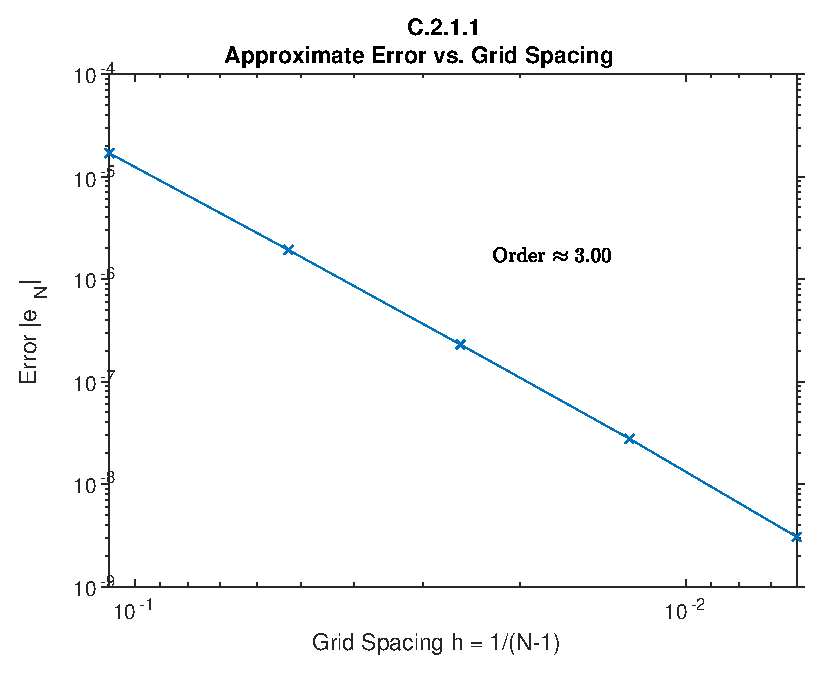
\includegraphics [width=4in]{lab2_06.eps}

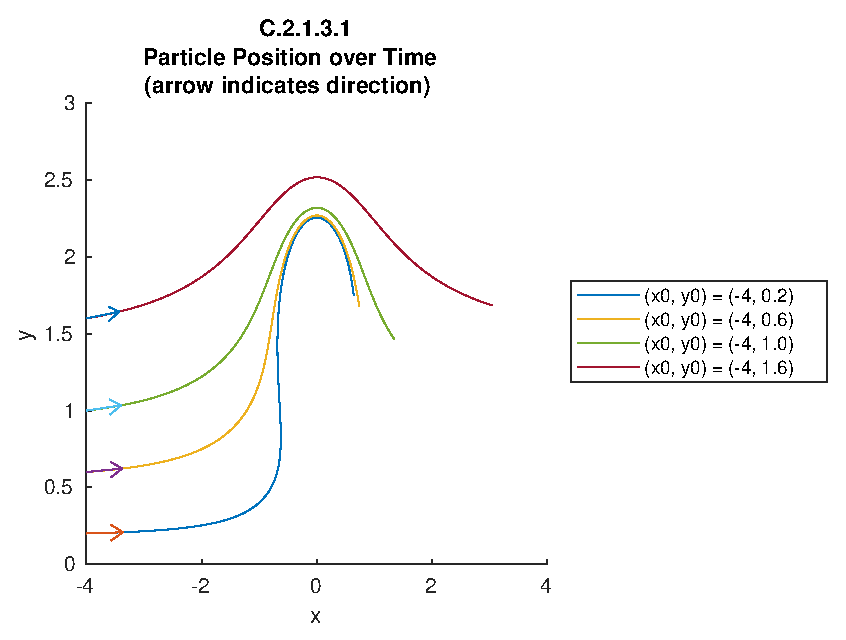
\includegraphics [width=4in]{lab2_07.eps}

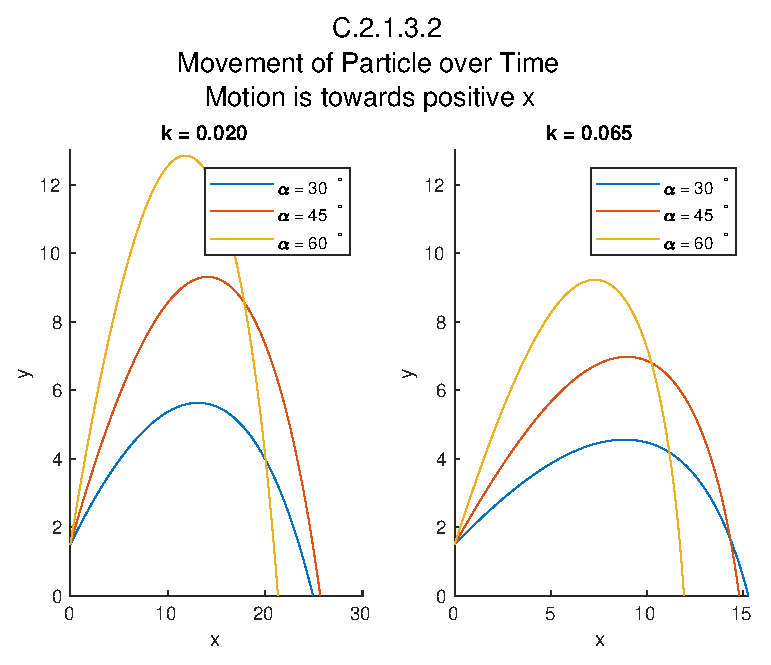
\includegraphics [width=4in]{lab2_08.eps}


\subsection*{Functions Used Above}

\begin{par}
In a matlab script file, all functions must be defined below the body of the script. As a result, a lot of the code that would be useful to read before reading the above is instead down here...
\end{par} \vspace{1em}
\begin{par}
Also, any figures that depend on the result of calling a function down here is also inherently delayed until this section has completed, often clustering output figures at the bottom of the file instead of inline with their corresponding section. :(
\end{par} \vspace{1em}


\subsection*{RK-3 Solver}

\begin{par}
This implements the explicit RK-3 scheme described in section ``Numerical Scheme.'' This solver assumes an IVP on a first order ODE of the form: $\bm{X}_t = f(t, \bm{X}), \quad \bm{X}(0) = \bm{X}_0$.
\end{par} \vspace{1em}
\begin{verbatim}
function [X, T, h] = rk3_solve(f, X_0, T_int, N)
% RK3_SOLVE solves the ODE X' = f(t, X) on the interval of t speicifed by
%           T_int. Uses X(T_int(1)) = X_0 as the initial condition at the
%           left endpoint of T_int. The approximate numerical solution will
%           have N points.
%           Parameters:
%             f     - the function on the RHS of the ODE (X' = f(t, X)).
%             X_0   - the initial data at the left endpoint of the support.
%             T_int - the two endpoints of the support.
%           Returns:
%             X - the numerical approximation of the function X.
%             T - the support for X.
%             h - the grid spacing of T.

% We expect X_0 to be a column vector, so let's reshape if needed.
X_0 = reshape(X_0, numel(X_0), 1);

% Generate the support as N linearly spaced points along the specified
% interval.
T = linspace(T_int(1), T_int(2), N);
h = T(2) - T(1);  % h is the spacing of the above linear partition.
% Allocate space for the solution as N columns of the size of X_0.
X = zeros(length(X_0), N);
X(:, 1) = X_0;  % Initialize with the boundary condition at T(1).

% Loop through all indices k for which we do not have a numerical
% approximation of X. NOTE: k = 1 is the initial condition.
for k = 2:N
    % Compute the values of K^{(k)}_{1,2,3} for this value of k.
    K = zeros(size(X, 1), 3);
    K(:, 1) = f(T(k-1), X(:, k-1));
    K(:, 2) = f(T(k-1) + h, X(:, k-1) + h*K(:, 1));
    K(:, 3) = f(T(k-1) + h/2, X(:, k-1) + h/4 * sum(K(:, 1:2), 2));

    % Compute the next value of the approximate solution.
    X(:, k) = X(:, k-1) + h/6 * sum(bsxfun(@times, [1 1 4], K), 2);
end

end
\end{verbatim}


\subsection*{RK-4 Solver}

\begin{par}
This implements the classic explicit RK-4 solver. Used in section C.2.1.3 where I am asked to choose a solver of at least order 2 to use.
\end{par} \vspace{1em}
\begin{verbatim}
function [X, T, h] = rk4_solve(f, X_0, T_int, N)
% RK4_SOLVE solves the ODE X' = f(t, X) on the interval of t speicifed by
%           T_int. Uses X(T_int(1)) = X_0 as the initial condition at the
%           left endpoint of T_int. The approximate numerical solution will
%           have N points.
%           Parameters:
%             f     - the function on the RHS of the ODE (X' = f(t, X)).
%             X_0   - the initial data at the left endpoint of the support.
%             T_int - the two endpoints of the support.
%           Returns:
%             X - the numerical approximation of the function X.
%             T - the support for X.
%             h - the grid spacing of T.

% We expect X_0 to be a column vector, so let's reshape if needed.
X_0 = reshape(X_0, numel(X_0), 1);

% Generate the support as N linearly spaced points along the specified
% interval.
T = linspace(T_int(1), T_int(2), N);
h = T(2) - T(1);  % h is the spacing of the above linear partition.
% Allocate space for the solution as N columns of the size of X_0.
X = zeros(length(X_0), N);
X(:, 1) = X_0;  % Initialize with the boundary condition at T(1).

% Loop through all indices k for which we do not have a numerical
% approximation of X. NOTE: k = 1 is the initial condition.
for k = 2:N
    % Compute the values of K^{(k)}_{1,2,3,4} for this value of k.
    K = zeros(size(X, 1), 4);
    K(:, 1) = f(T(k-1), X(:, k-1));
    K(:, 2) = f(T(k-1) + h/2, X(:, k-1) + h/2*K(:, 1));
    K(:, 3) = f(T(k-1) + h/2, X(:, k-1) + h/2*K(:, 2));
    K(:, 4) = f(T(k-1) + h, X(:, k-1) + h*K(:, 3));

    % Compute the next value of the approximate solution.
    X(:, k) = X(:, k-1) + h/6 * sum(bsxfun(@times, [1 2 2 1], K), 2);
end

end
\end{verbatim}



\end{document}
    
